\begin{figure*}[t]
\centering
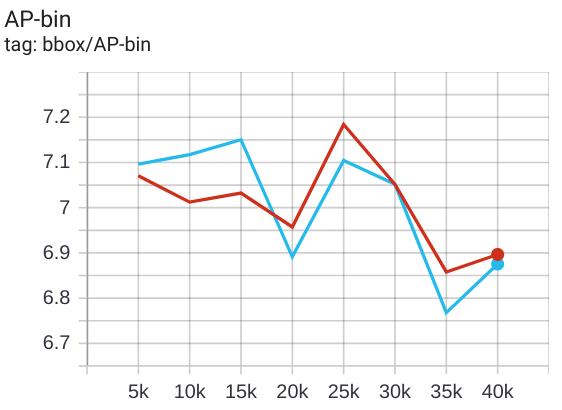
\includegraphics[width=0.6\textwidth]{fig/ap.png}
\vspace{-0.35cm}
\caption{AP on the test dataset during training}
\vspace{-0.4cm}
\label{fig:ap}
\end{figure*}

\begin{figure*}[t]
\centering
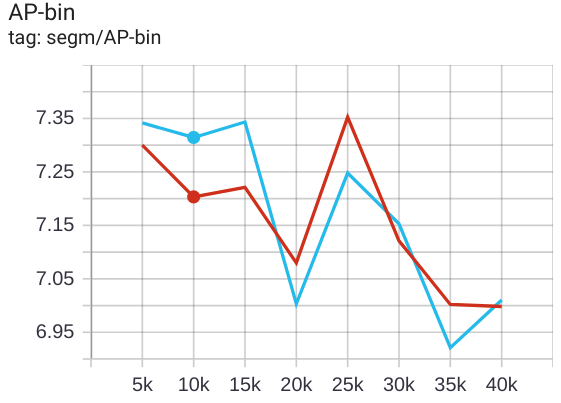
\includegraphics[width=0.6\textwidth]{fig/ap_bin_s.png}
\vspace{-0.35cm}
\caption{AP for object class 'bin' on the test dataset during training}
\vspace{-0.4cm}
\label{fig:ap_bin}
\end{figure*}

\begin{figure*}[t]
\centering
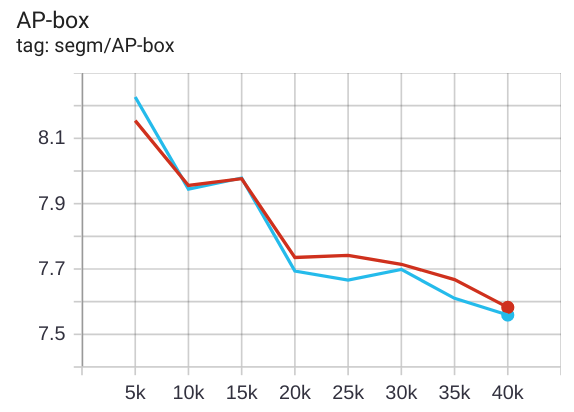
\includegraphics[width=0.6\textwidth]{fig/ap_box_s.png}
\vspace{-0.35cm}
\caption{AP for object class 'box' on the test dataset during training}
\vspace{-0.4cm}
\label{fig:ap_box}
\end{figure*}

\begin{figure*}[t]
\centering
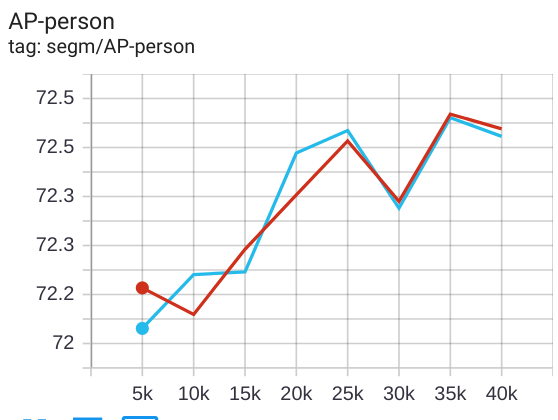
\includegraphics[width=0.6\textwidth]{fig/ap_person_s.png}
\vspace{-0.35cm}
\caption{AP for object class 'person' on the test dataset during training}
\vspace{-0.4cm}
\label{fig:ap_person}
\end{figure*}

